% !TEX program = xelatex
\documentclass[
  10pt,
  twoside,
  openany,
  b5paper, % 以上均为 ctexbook 提供的文类选项
  colorscheme = basic, % 请根据需要选择或定制配色方案
]{qyxf-book}

\usepackage[contents = 钱院学辅, scale = 15, color = black, angle = 50, opacity = .10]{background}
\usepackage{pdfpages}
\includepdfset{pagecommand={\thispagestyle{plain}}}

\title{电磁场与波课件与笔记}
\subtitle{Slides and Notes of Electromagnetic Field and Waves}  % 可选
\author{邹建龙\ 电气钱82班蔡易骎}
\date{2021 年 1 月 28 日}

% 定制元信息
\org{\Large\textit{钱学森书院学业辅导中心}\\\textsc{Qian Xuesen College Academic Counseling Center}}
\footorg{\textsc{Qian Yuan Xue Fu}}
\cover{
	\begin{tikzpicture}[remember picture, overlay]
		\begin{pgfonlayer}{background}
			\node at ($(current page.east)+(0in,0in)$){
				
\includegraphics[width=.8\textwidth]{cover.png} };
		\end{pgfonlayer}
	\end{tikzpicture}
}
\license{}  % 清空许可证信息

% 调整封面标题大小
\renewcommand{\titlefont}{\Huge\bfseries}
\renewcommand{\subtitlefont}{\LARGE\itshape}

\begin{document}

\maketitle

\chapter*{前言}
\thispagestyle{empty}

电磁场作为电气专业的“四大名补”,难度不言而喻.学习电磁场的感觉有点虚无缥缈,因为这些东西是很抽象的,看不见摸不着,像是凭空想象再加上一堆复杂的数学推导得出的结果.

因为电磁场这门课程如此的特点,我觉得在学习的过程中对一些概念和结论的记忆反而更加重要.

对于一些很长很复杂的公式,或许因为考试的缘故我们需要硬着头皮背下来,但在学习的过程中可以关注一下推导过程.这里的推导过程当然不是指复杂的数学恒等式变换,而是关注几个问题,例如”推导用到了前面学习的哪些知识”,”是哪个公式结合另一个得来的”,”这个公式想说明什么”,”同构这个公式我可以由哪些条件计算出我要的结果”等等.有了这些思考,理解可能会更加深刻,背起来也不那么痛苦了.关于这点,典型的例子应该是坡印廷定理的物理意义了.

然后应该有自己的一点收获,这也是我们学习的目的之一.这些很难很长的公式我们考完试之后应该是记不住的,需要的可能是以后要用的时候能够记得当初学过,知道大概的意思,查阅资料后能够正确使用.这也是我觉得一些概念的东西反而更加重要的原因,当然一些重要的结论能记得也是很用帮助的.

\rightline{——电气钱82班\ 蔡易骎} 

\newpage
\tableofcontents

\newpage
\addcontentsline{toc}{chapter}{1 电磁场数学基础}
\includepdf[pages = - , nup=2x3]{content/1 电磁场数学基础(笔记).pdf}
\addcontentsline{toc}{chapter}{2 真空中的静电场描述}
\includepdf[pages = - , nup=2x3]{content/2 真空中的静电场描述(笔记).pdf}
\addcontentsline{toc}{chapter}{3 静电场的方程和求解(1)}
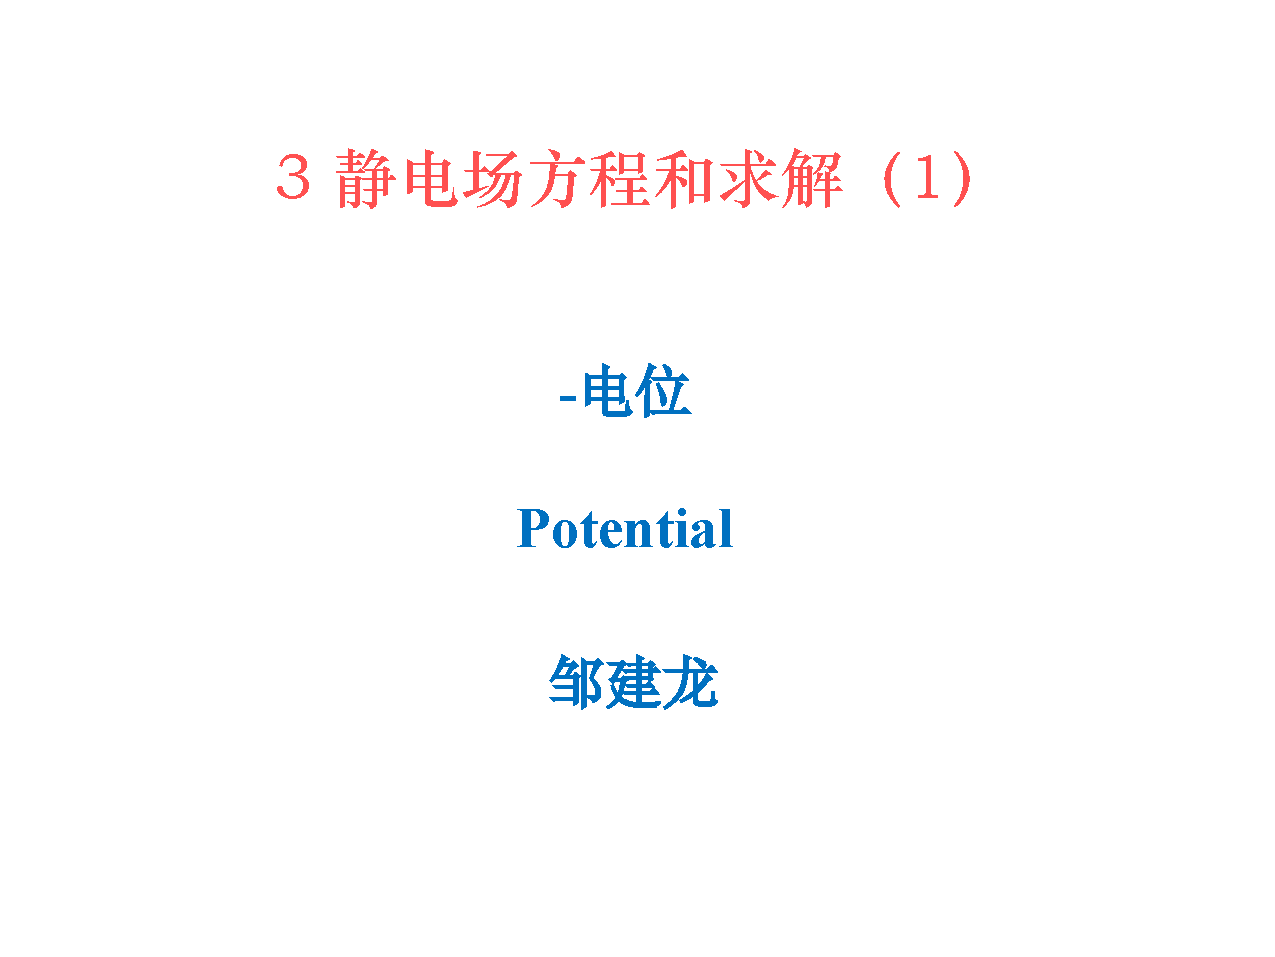
\includepdf[pages = - , nup=2x3]{content/3 静电场的方程和求解(1)(笔记).pdf}
\addcontentsline{toc}{chapter}{4 静电场的方程和求解(2)}
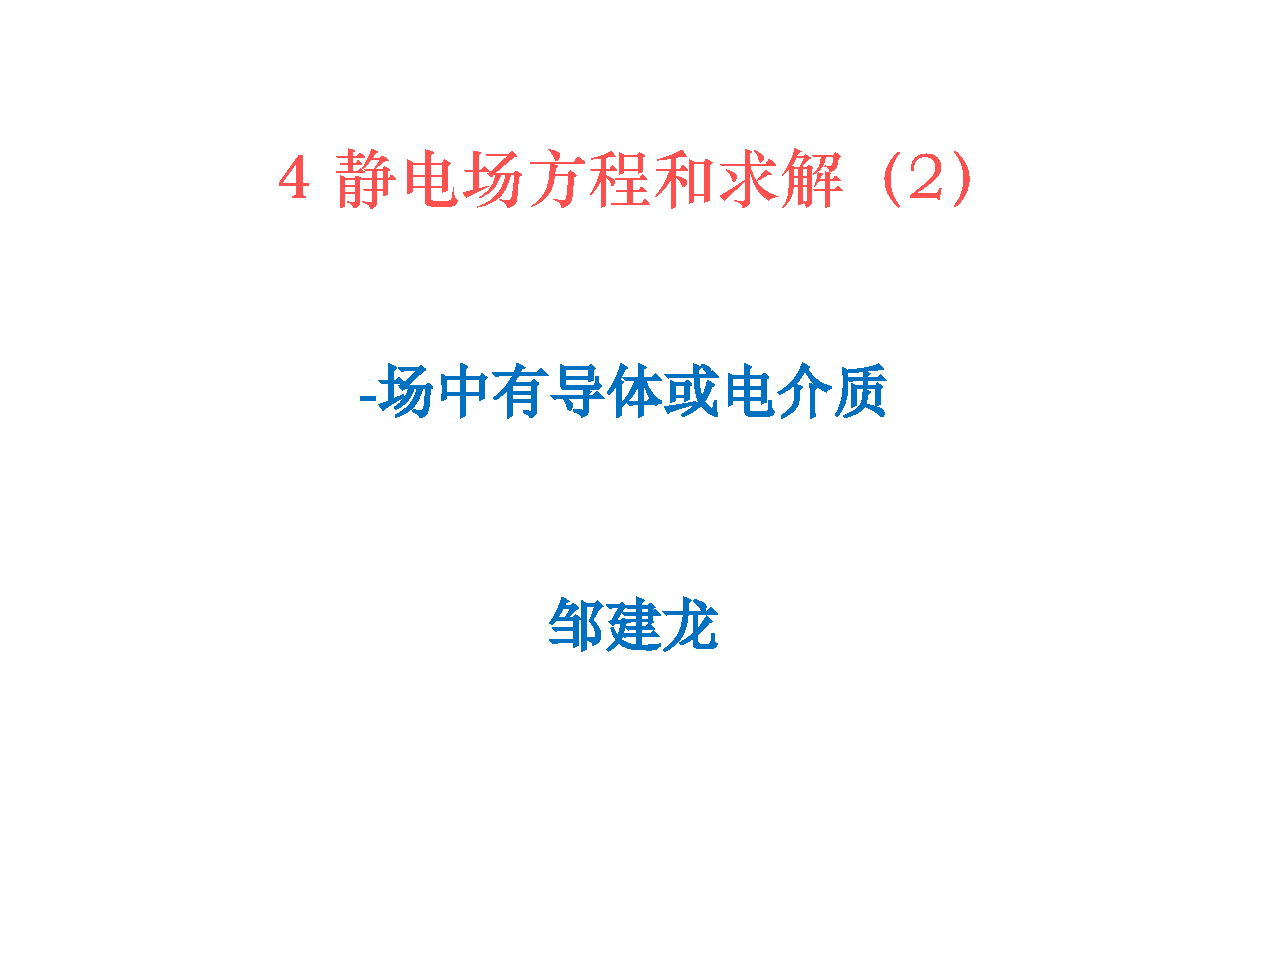
\includepdf[pages = - , nup=2x3]{content/4 静电场的方程和求解(2)(笔记).pdf}
\addcontentsline{toc}{chapter}{5 静电场的方程和求解(3)}
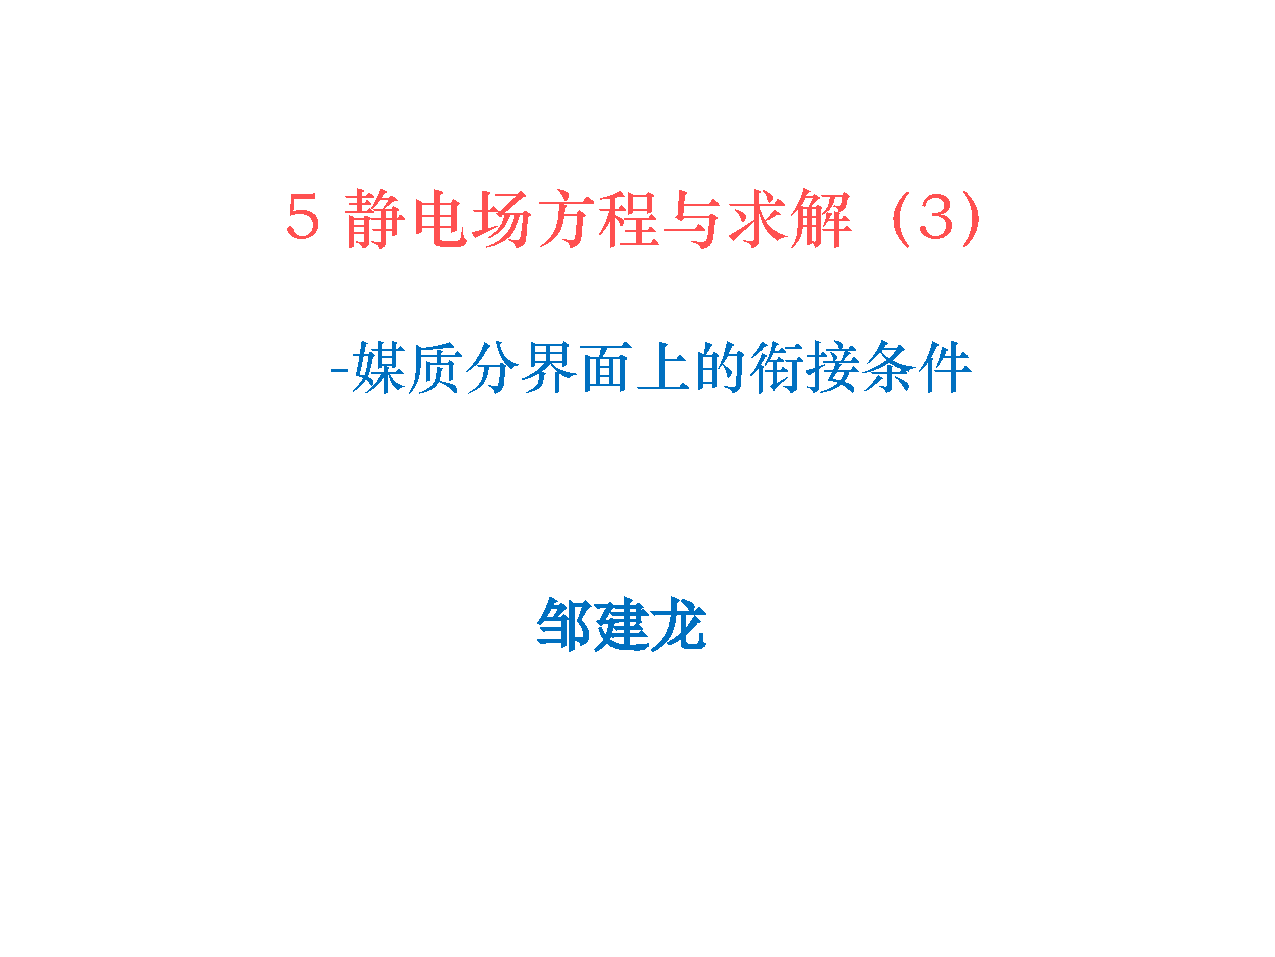
\includepdf[pages = - , nup=2x3]{content/5 静电场的方程和求解(3)(笔记).pdf}
\addcontentsline{toc}{chapter}{6 泊松方程、拉普拉斯方程、边值问题及其求解}
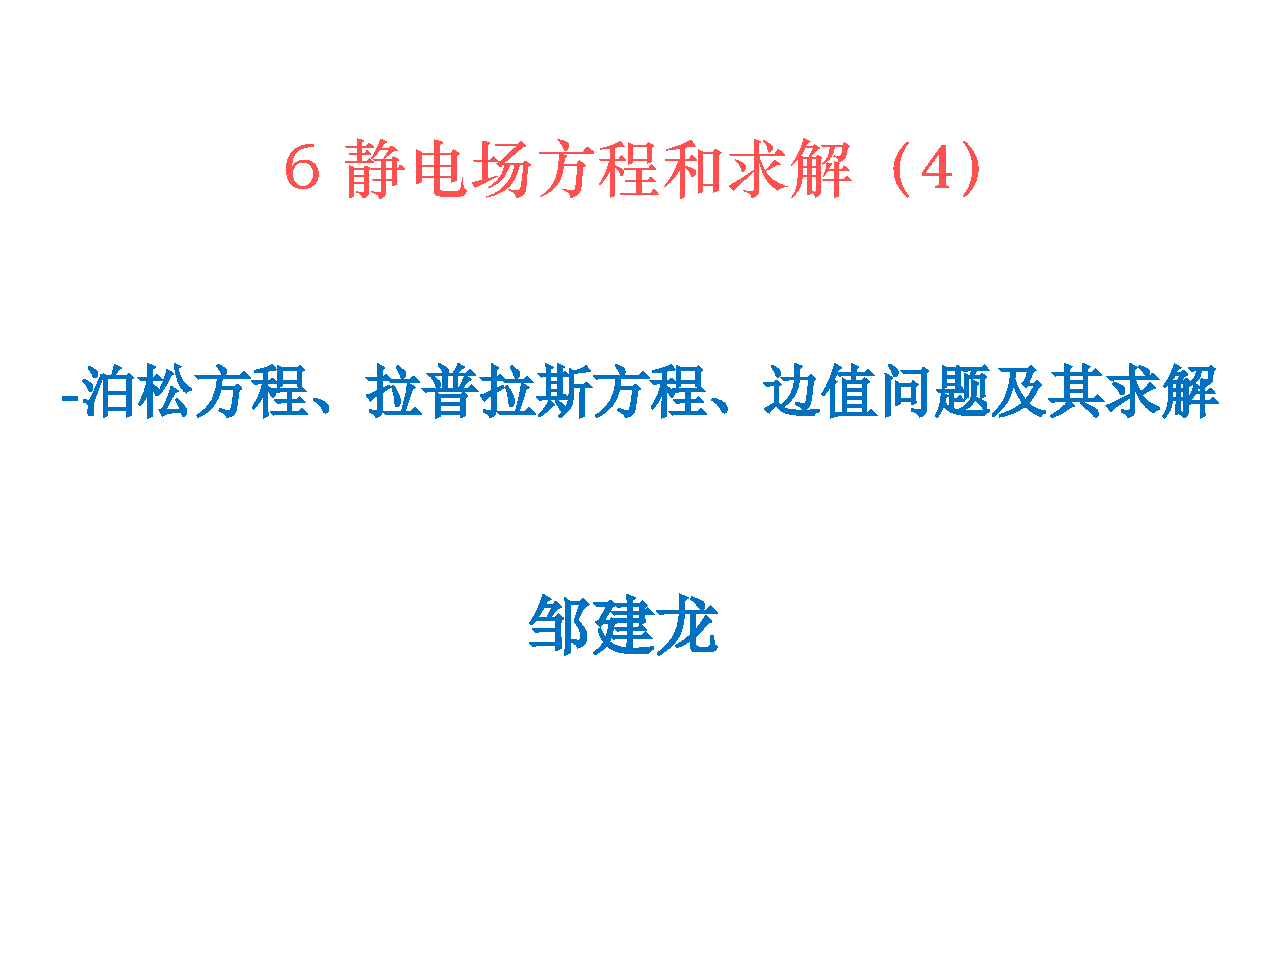
\includepdf[pages = - , nup=2x3]{content/6 泊松方程、拉普拉斯方程、边值问题及其求解(笔记).pdf}
\addcontentsline{toc}{chapter}{7 静电场的方程和求解(5)-唯一性定理和分离变量法}
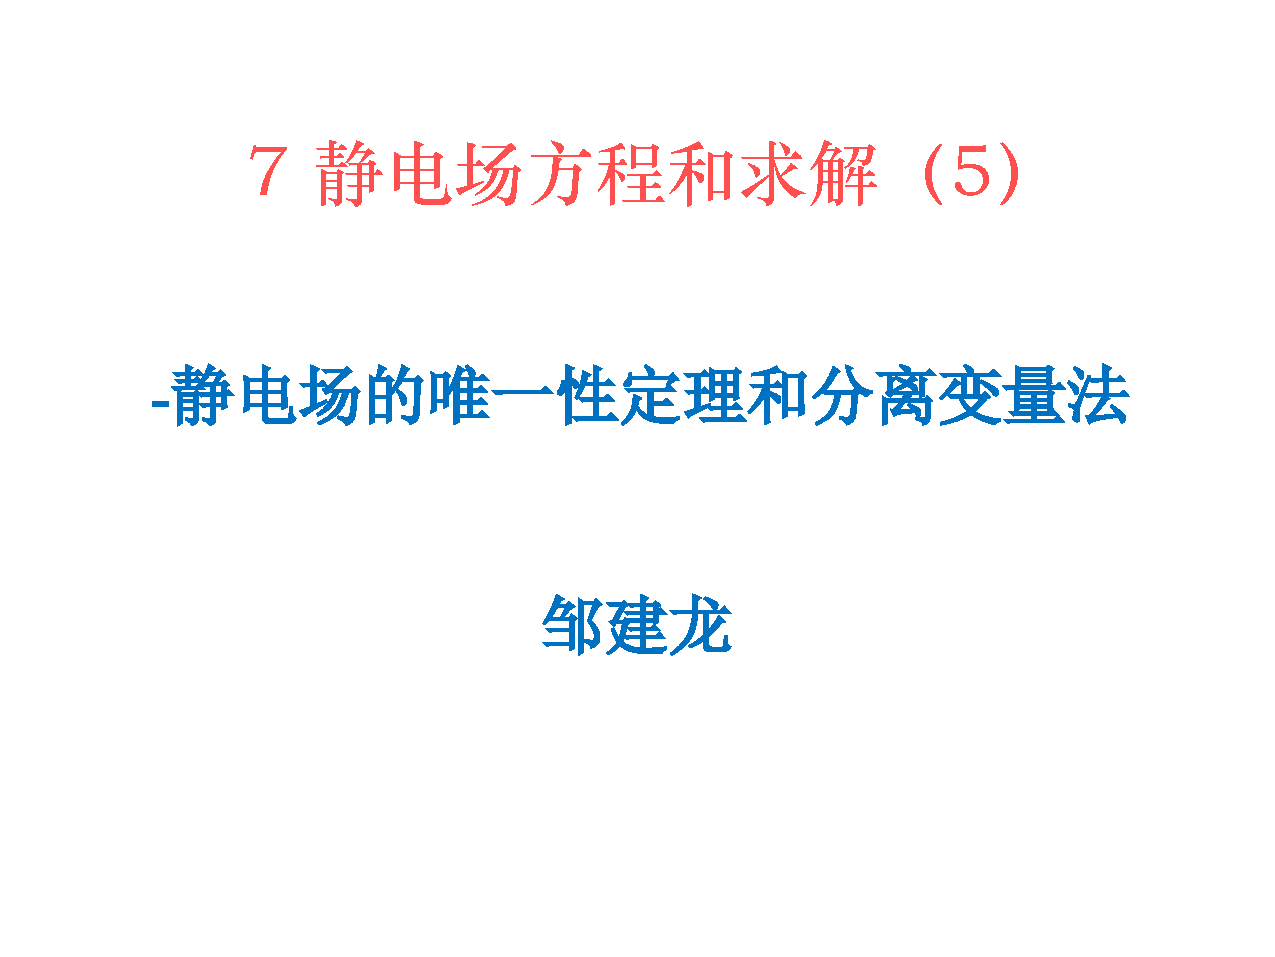
\includepdf[pages = - , nup=2x3]{content/7 静电场的方程和求解(5)-唯一性定理和分离变量法(笔记).pdf}
\addcontentsline{toc}{chapter}{8 静电场的方程和求解(6)-镜像法和电轴法}
\includepdf[pages = - , nup=2x3]{content/8 静电场的方程和求解(6)-镜像法和电轴法(笔记)_部分1.pdf}
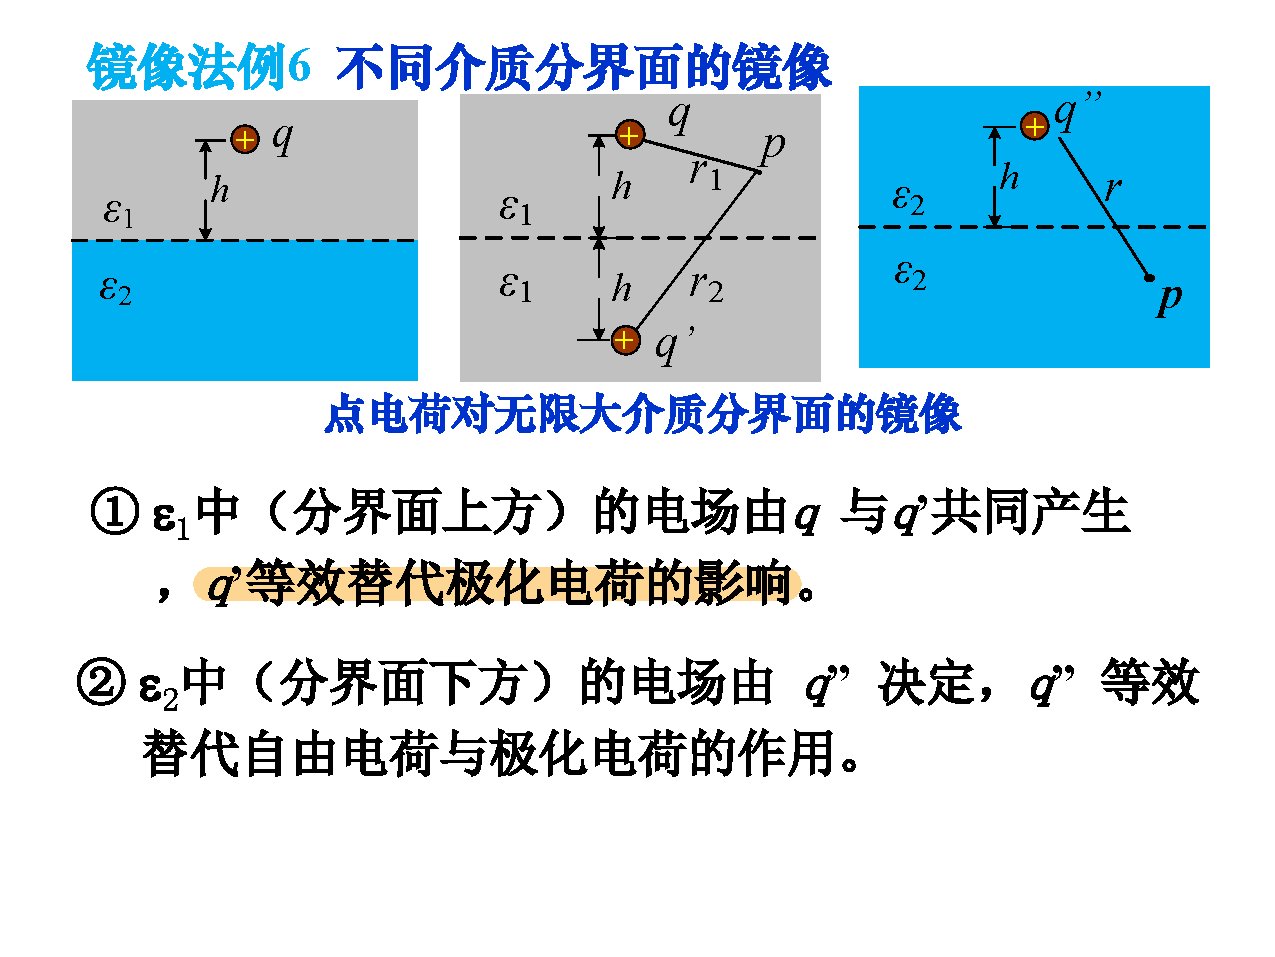
\includepdf[pages = - , nup=2x3]{content/8 静电场的方程和求解(6)-镜像法和电轴法(笔记)_部分2.pdf}
\addcontentsline{toc}{chapter}{9 静电场的应用-电容和部分电容}
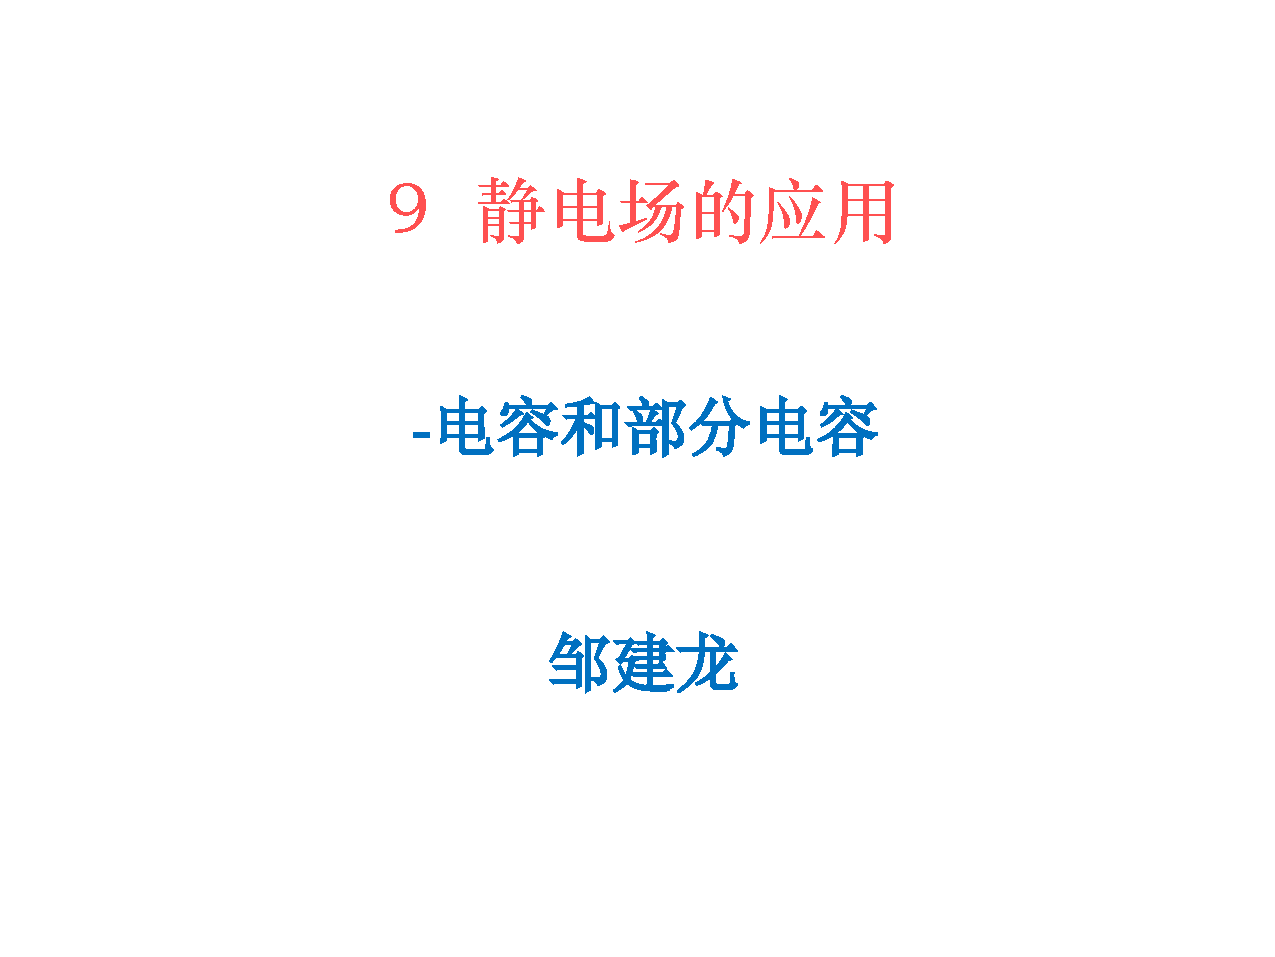
\includepdf[pages = - , nup=2x3]{content/9 静电场的应用-电容和部分电容(笔记).pdf}
\addcontentsline{toc}{chapter}{10 恒定电(流)场的定义和方程}
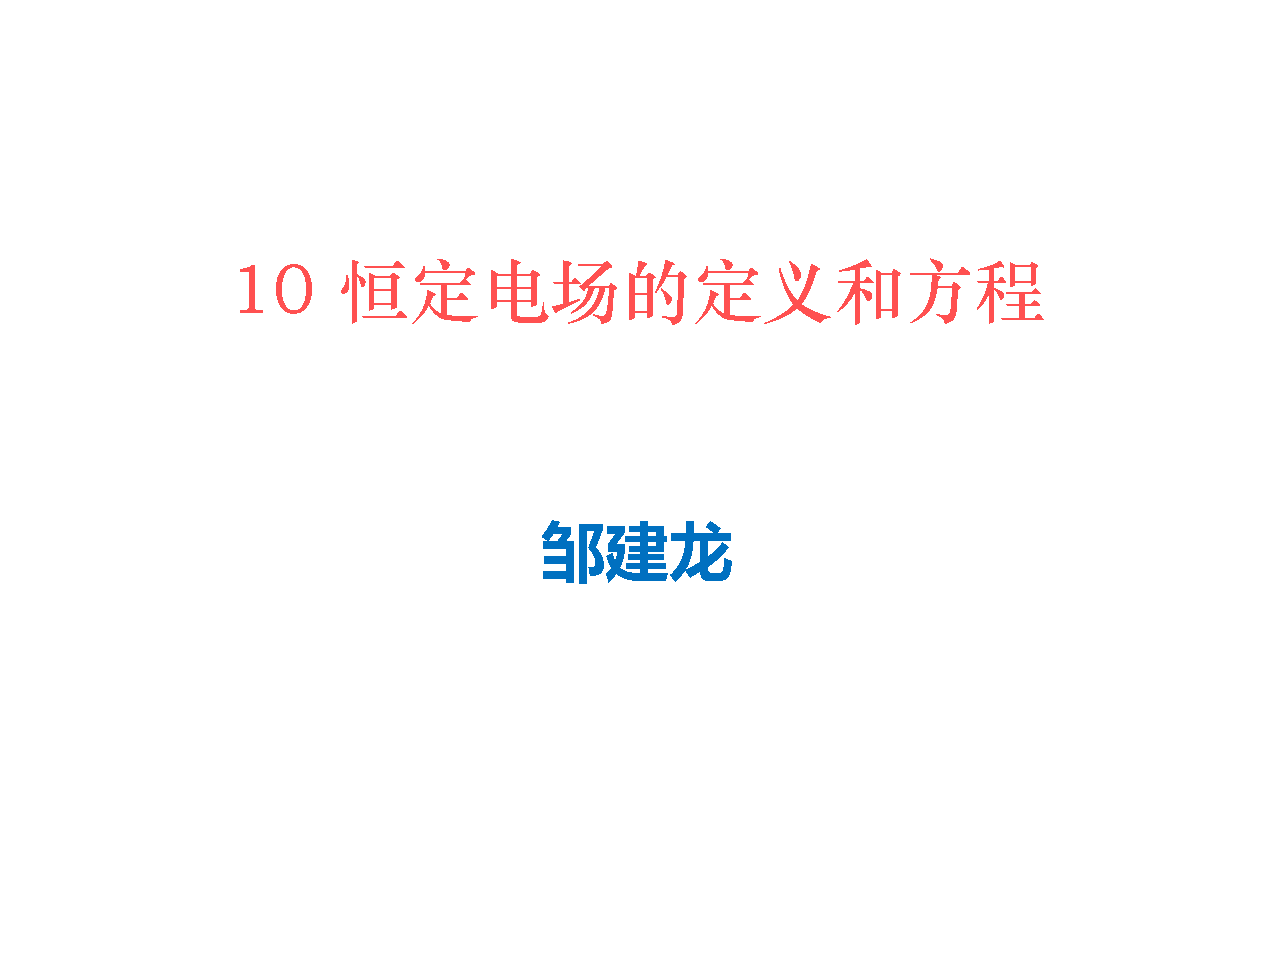
\includepdf[pages = - , nup=2x3]{content/10 恒定电(流)场的定义和方程(笔记).pdf}
\addcontentsline{toc}{chapter}{11 恒定电(流)场的分界面衔接条件和方程求解}
\includepdf[pages = - , nup=2x3]{content/11 恒定电(流)场的分界面衔接条件和方程求解.pdf}
\addcontentsline{toc}{chapter}{12 恒定电(流)场的应用-电导和部分电导}
\includepdf[pages = - , nup=2x3]{content/12 恒定电(流)场的应用-电导和部分电导(笔记).pdf}
\addcontentsline{toc}{chapter}{13 恒定磁场基本定律和方程}
\includepdf[pages = - , nup=2x3]{content/13 恒定磁场基本定律和方程(笔记).pdf}
\addcontentsline{toc}{chapter}{14 恒定磁场磁矢位的定义和计算}
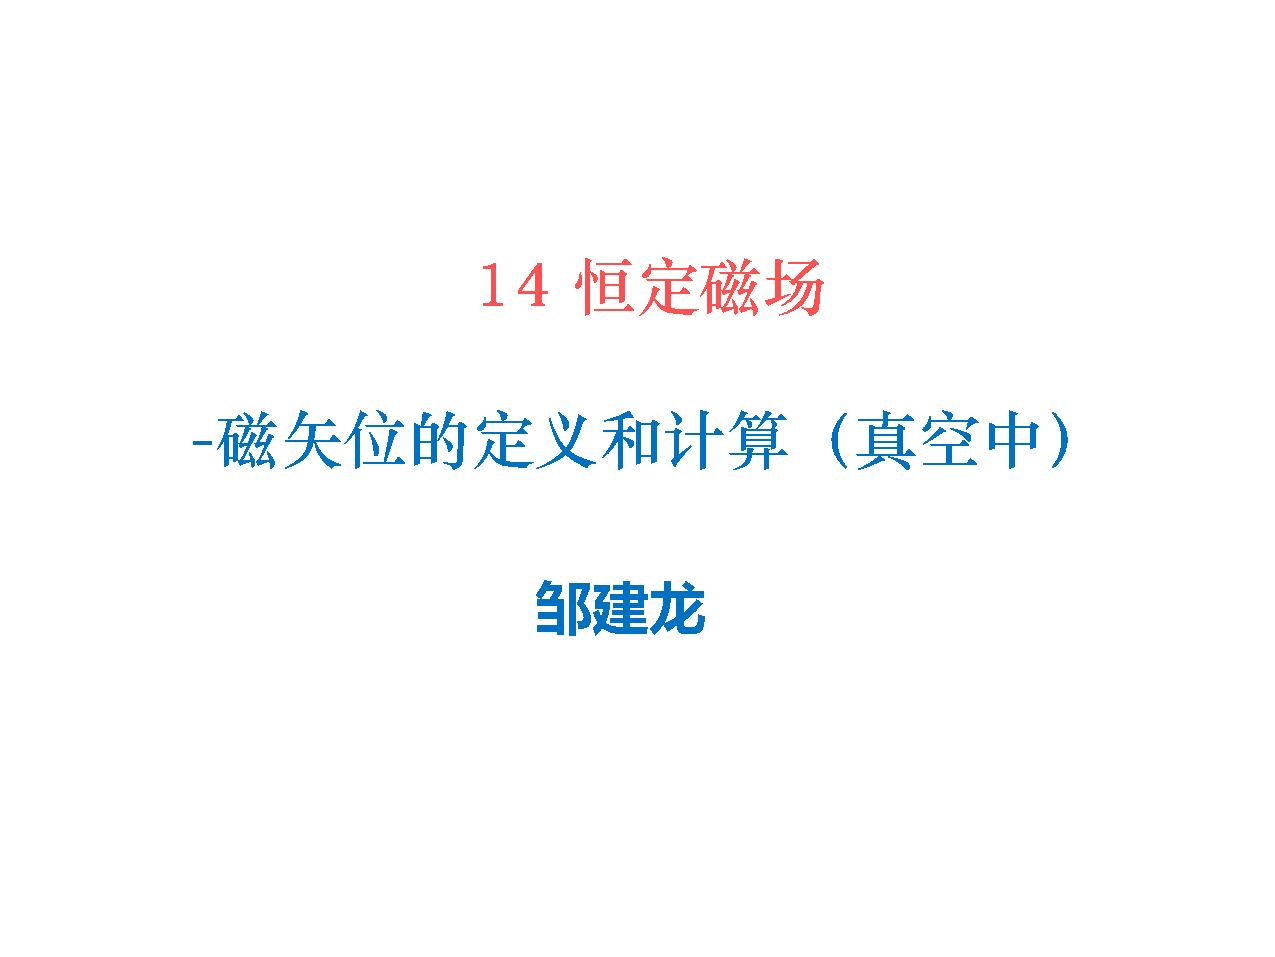
\includepdf[pages = - , nup=2x3]{content/14 恒定磁场磁矢位的定义和计算(笔记).pdf}
\addcontentsline{toc}{chapter}{15 恒定磁场-导磁材料的磁化}
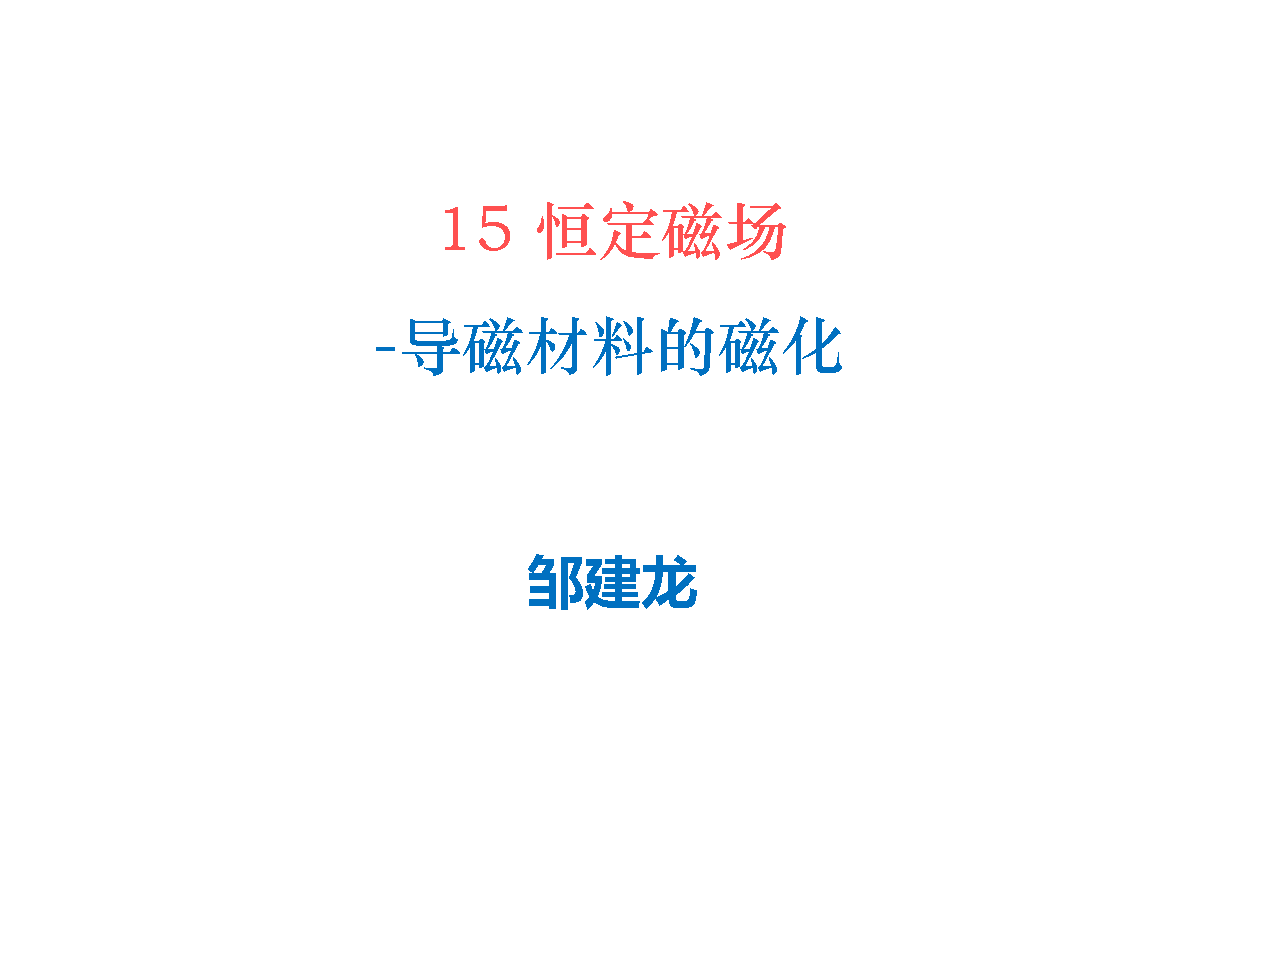
\includepdf[pages = - , nup=2x3]{content/15 恒定磁场-导磁材料的磁化(1).pdf}
\addcontentsline{toc}{chapter}{16 恒定磁场分界面衔接条件}
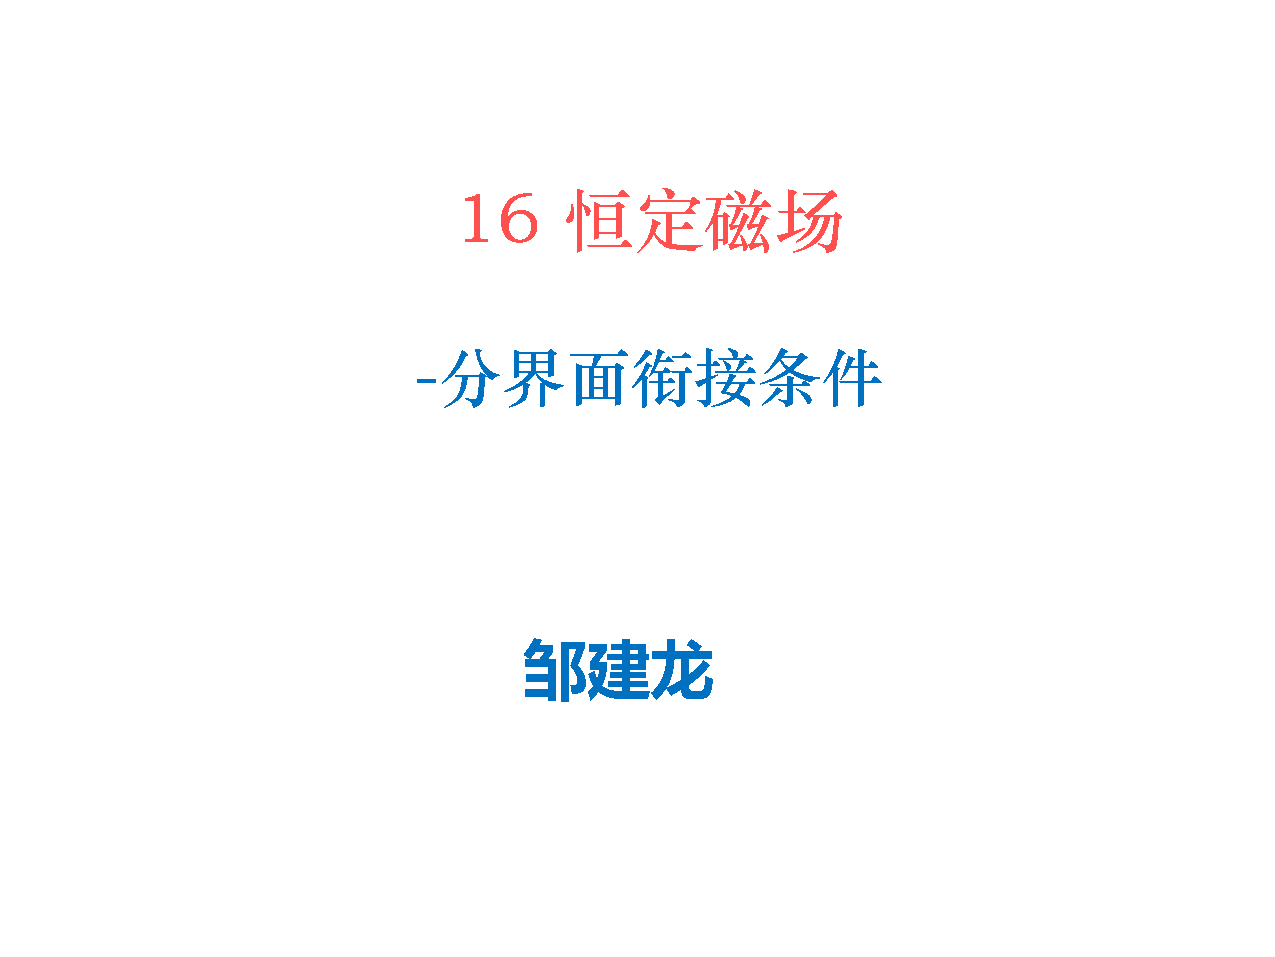
\includepdf[pages = - , nup=2x3]{content/16 恒定磁场分界面衔接条件.pdf}
\addcontentsline{toc}{chapter}{17 恒定磁场-镜像法}
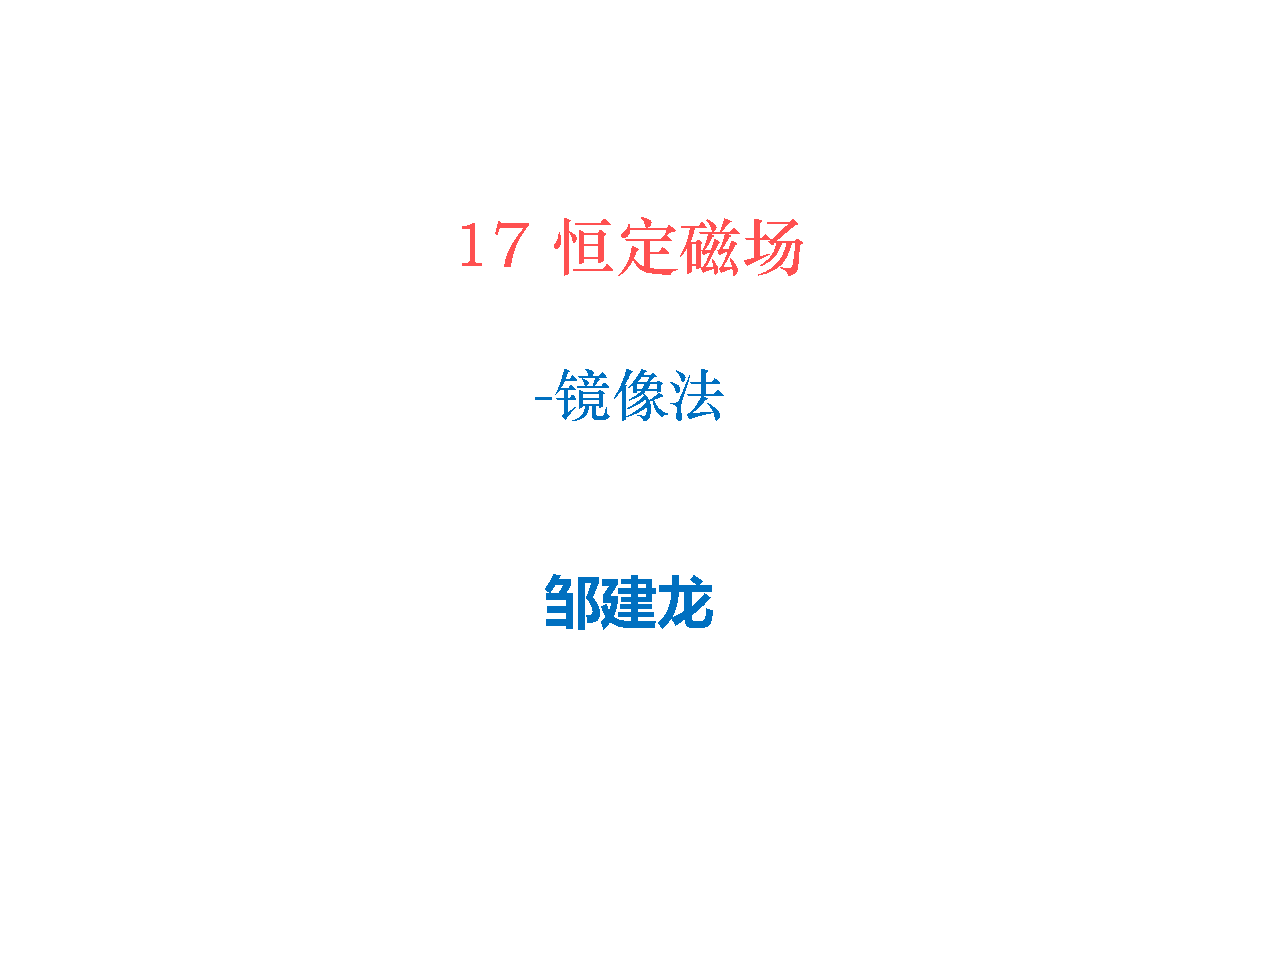
\includepdf[pages = - , nup=2x3]{content/17 恒定磁场-镜像法.pdf}
\addcontentsline{toc}{chapter}{18 恒定磁场-磁位、磁压、磁路}
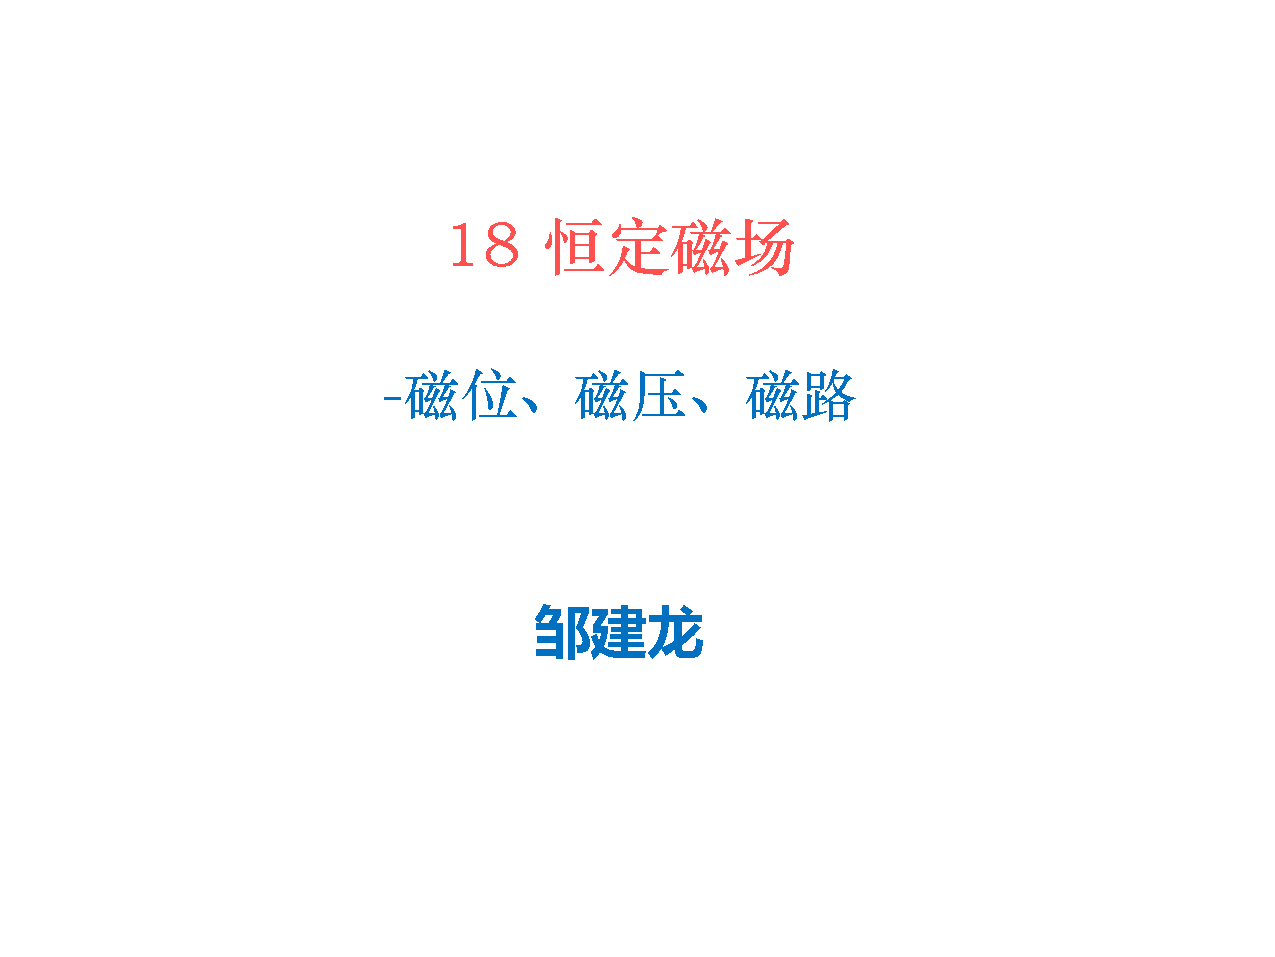
\includepdf[pages = - , nup=2x3]{content/18 恒定磁场-磁位、磁压、磁路.pdf}
\addcontentsline{toc}{chapter}{19 恒定磁场的应用-电感}
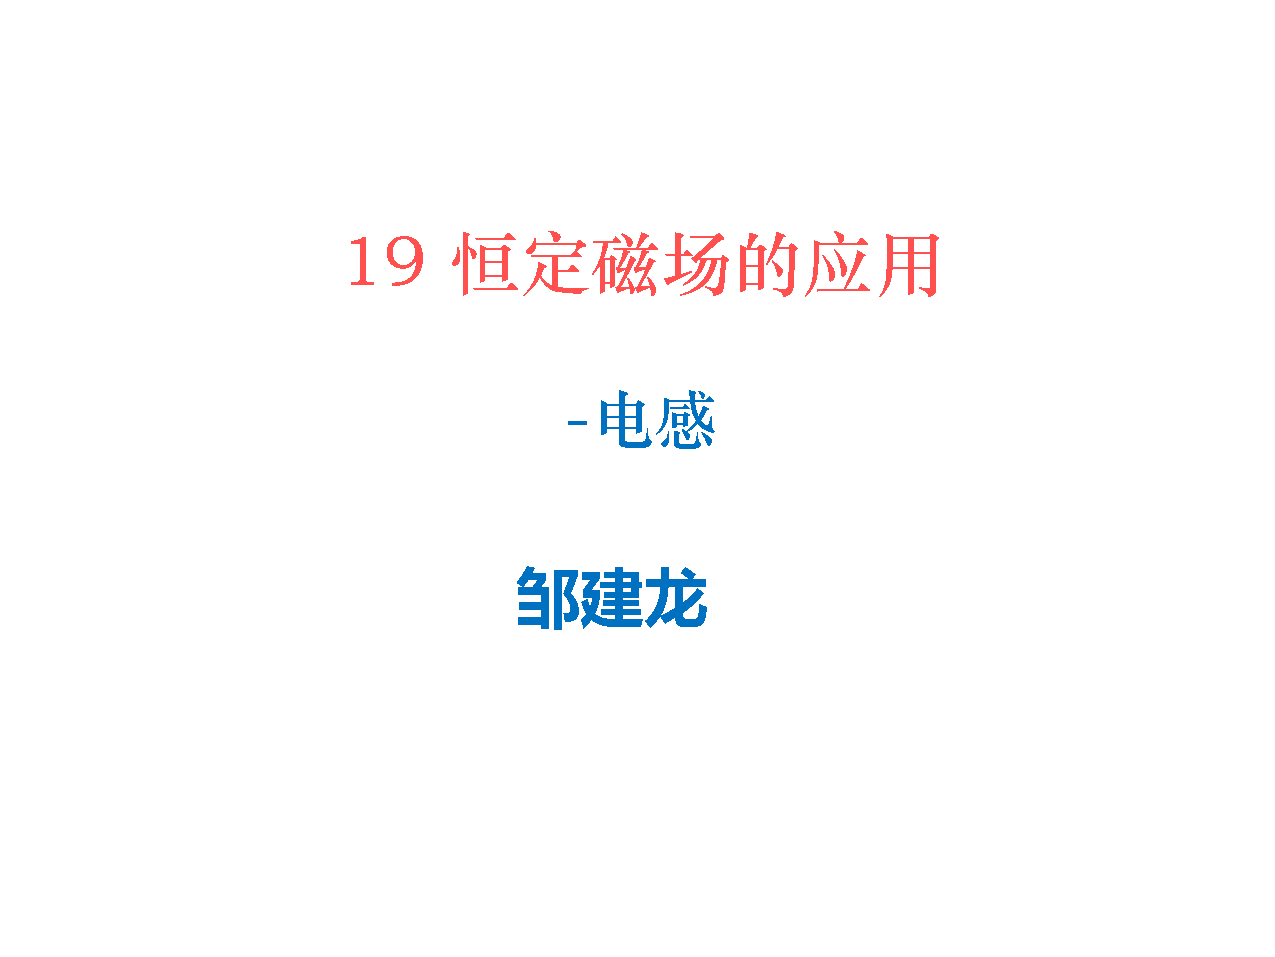
\includepdf[pages = - , nup=2x3]{content/19 恒定磁场的应用-电感(笔记).pdf}
\addcontentsline{toc}{chapter}{20 时变电磁场-麦克斯韦方程组和分界面衔接条件}
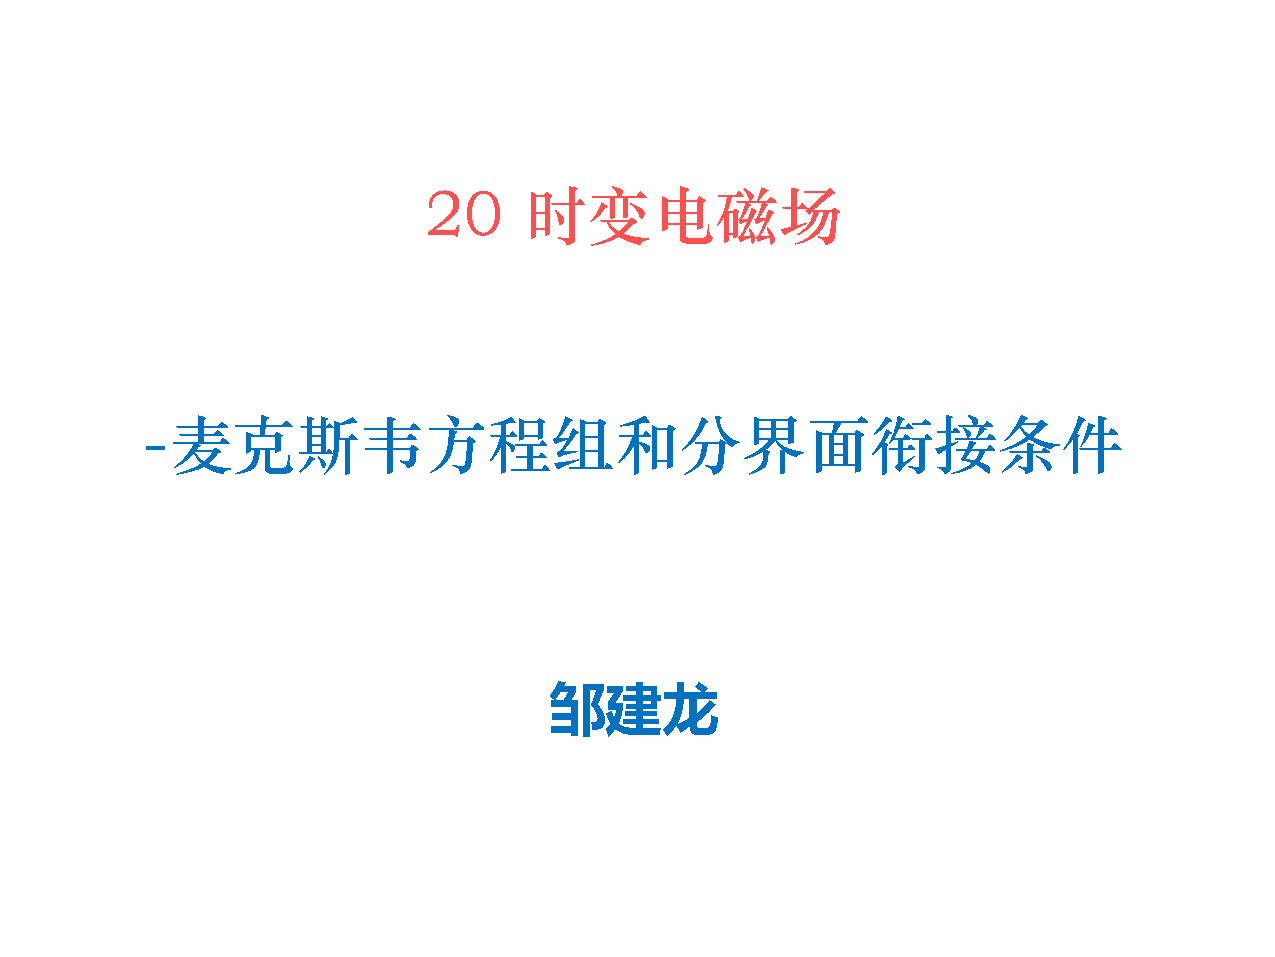
\includepdf[pages = - , nup=2x3]{content/20 时变电磁场-麦克斯韦方程组和分界面衔接条件.pdf}
\addcontentsline{toc}{chapter}{21 时变电磁场-动态位及其积分解}
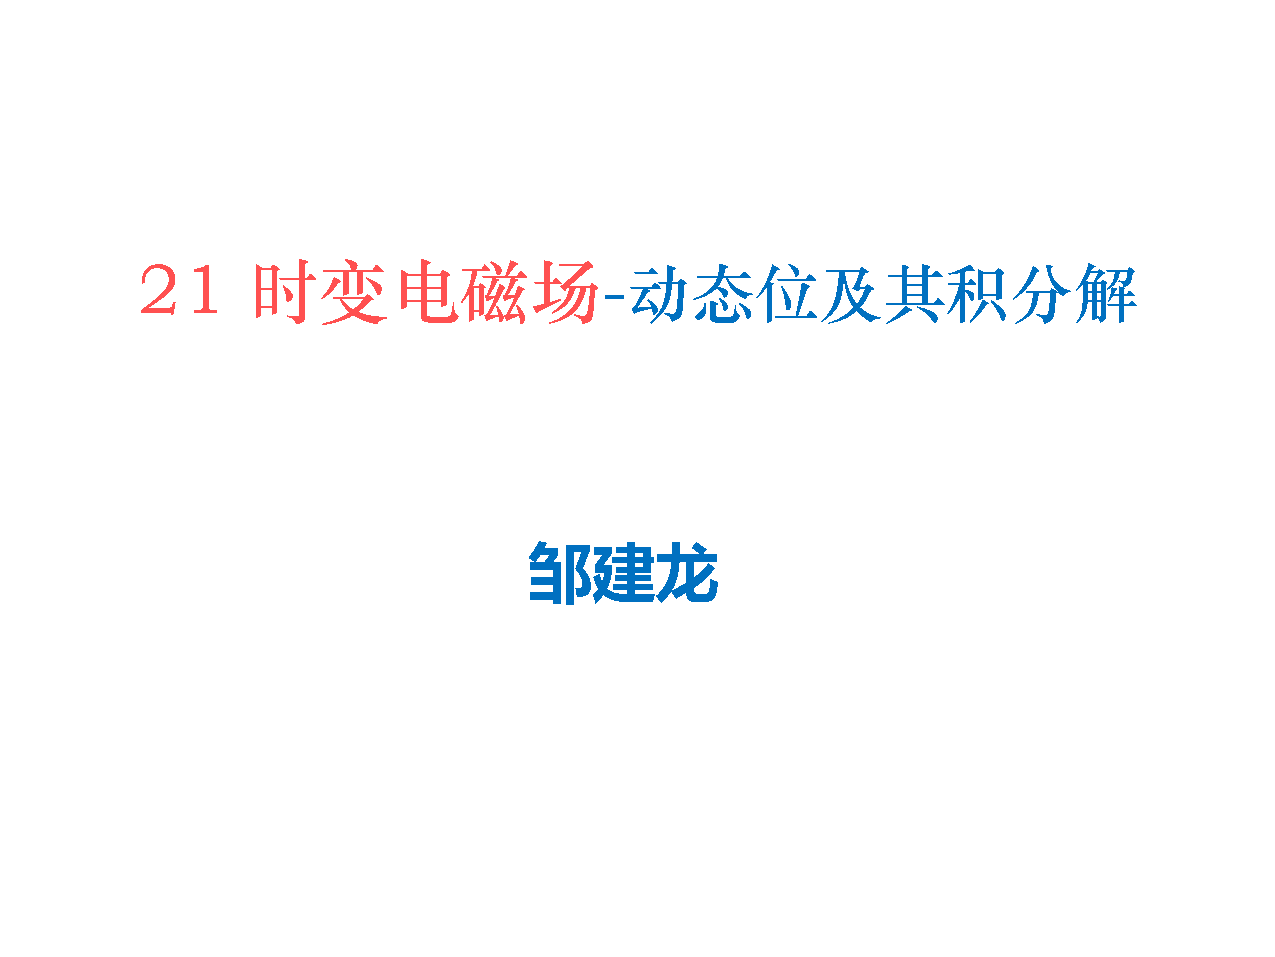
\includepdf[pages = - , nup=2x3]{content/21 时变电磁场-动态位及其积分解(笔记).pdf}
\addcontentsline{toc}{chapter}{22 时变电磁场-正弦电磁场}
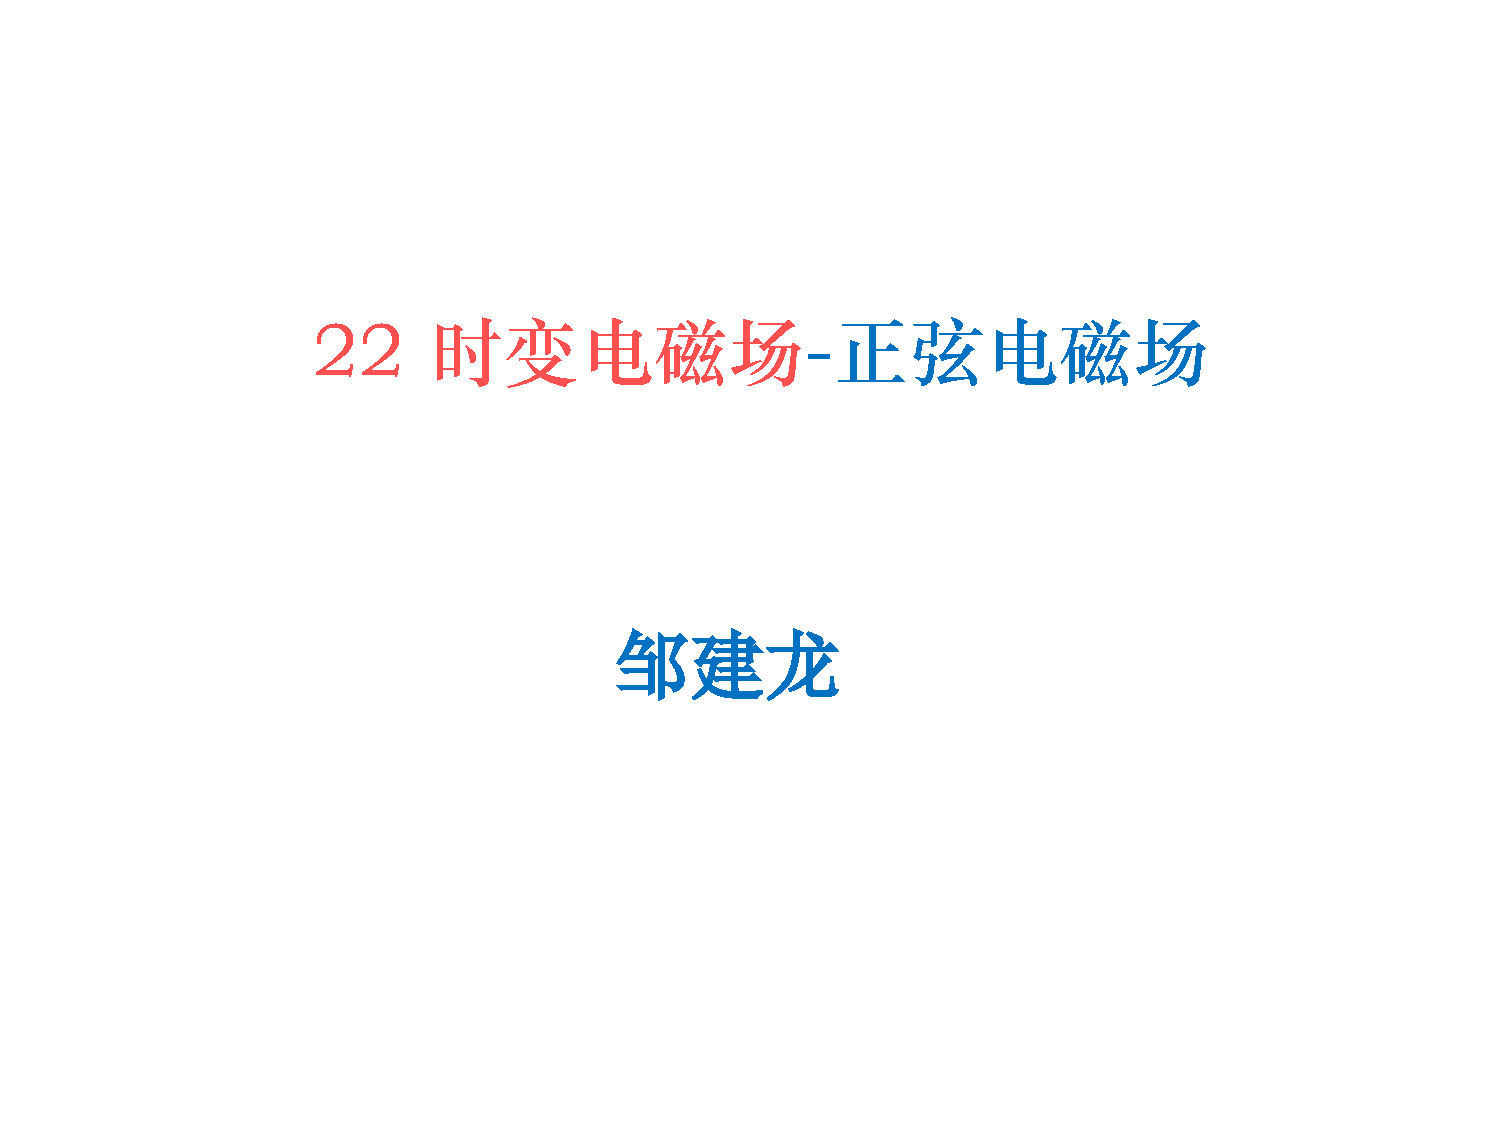
\includepdf[pages = - , nup=2x3]{content/22 时变电磁场-正弦电磁场.pdf}
\addcontentsline{toc}{chapter}{23 时变电磁场的应用-平面电磁波(1)-平面电磁波简介与方程}
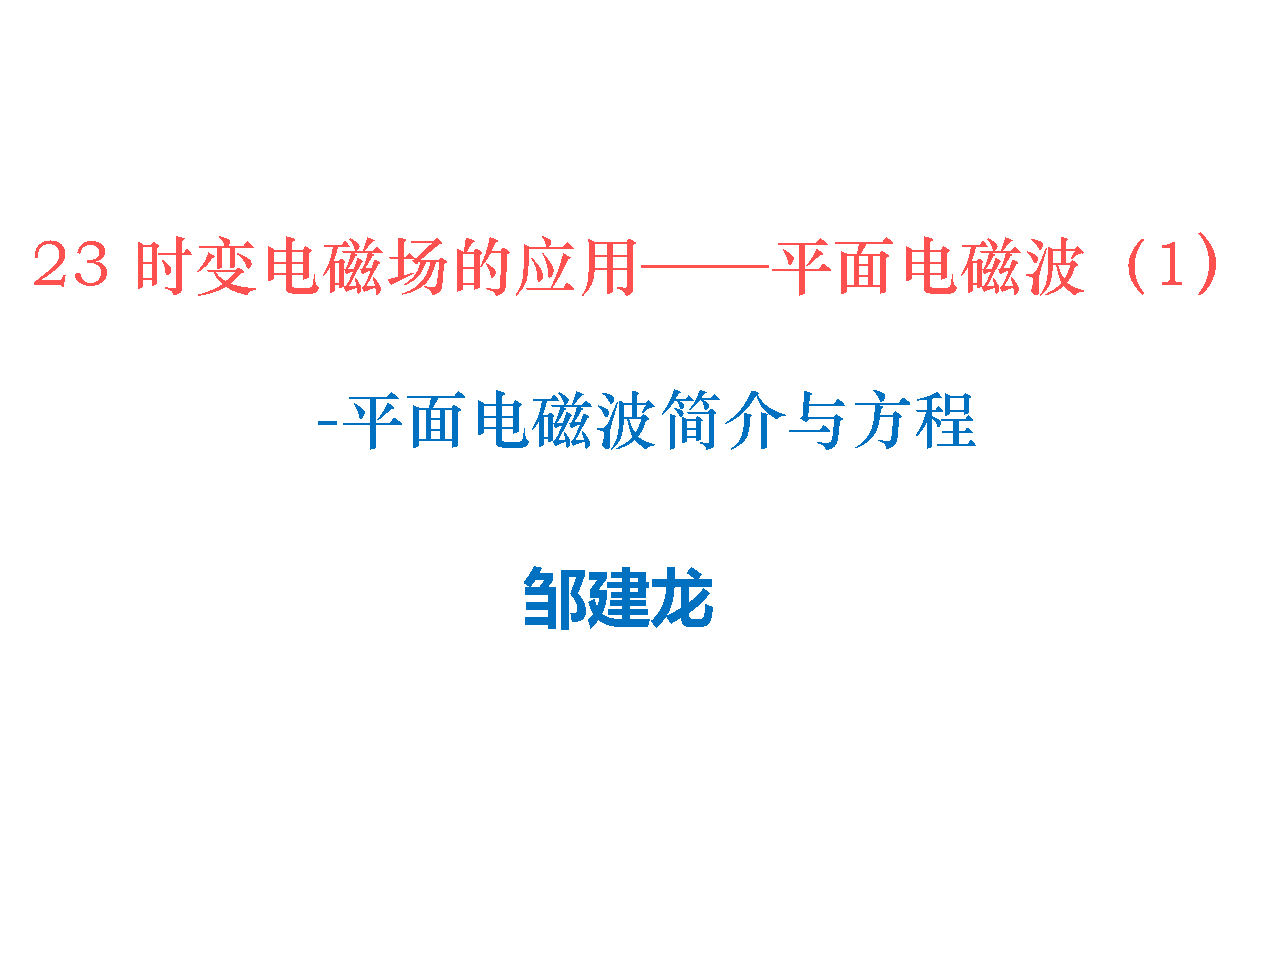
\includepdf[pages = - , nup=2x3]{content/23 时变电磁场的应用-平面电磁波(1)-平面电磁波简介与方程(笔记).pdf}
\addcontentsline{toc}{chapter}{24 时变电磁场的应用-平面电磁波(2)-理想介质中的均匀平面电磁波}
\includepdf[pages = - , nup=2x3]{content/24 时变电磁场的应用-平面电磁波(2)-理想介质中的均匀平面电磁波(笔记).pdf}
\addcontentsline{toc}{chapter}{25 时变电磁场的应用-平面电磁波(3)-导电媒质中的均匀平面电磁波}
\includepdf[pages = - , nup=2x3]{content/25 时变电磁场的应用-平面电磁波(3)-导电媒质中的均匀平面电磁波(笔记).pdf}
\addcontentsline{toc}{chapter}{26 时变电磁场-平面电磁波的极化}
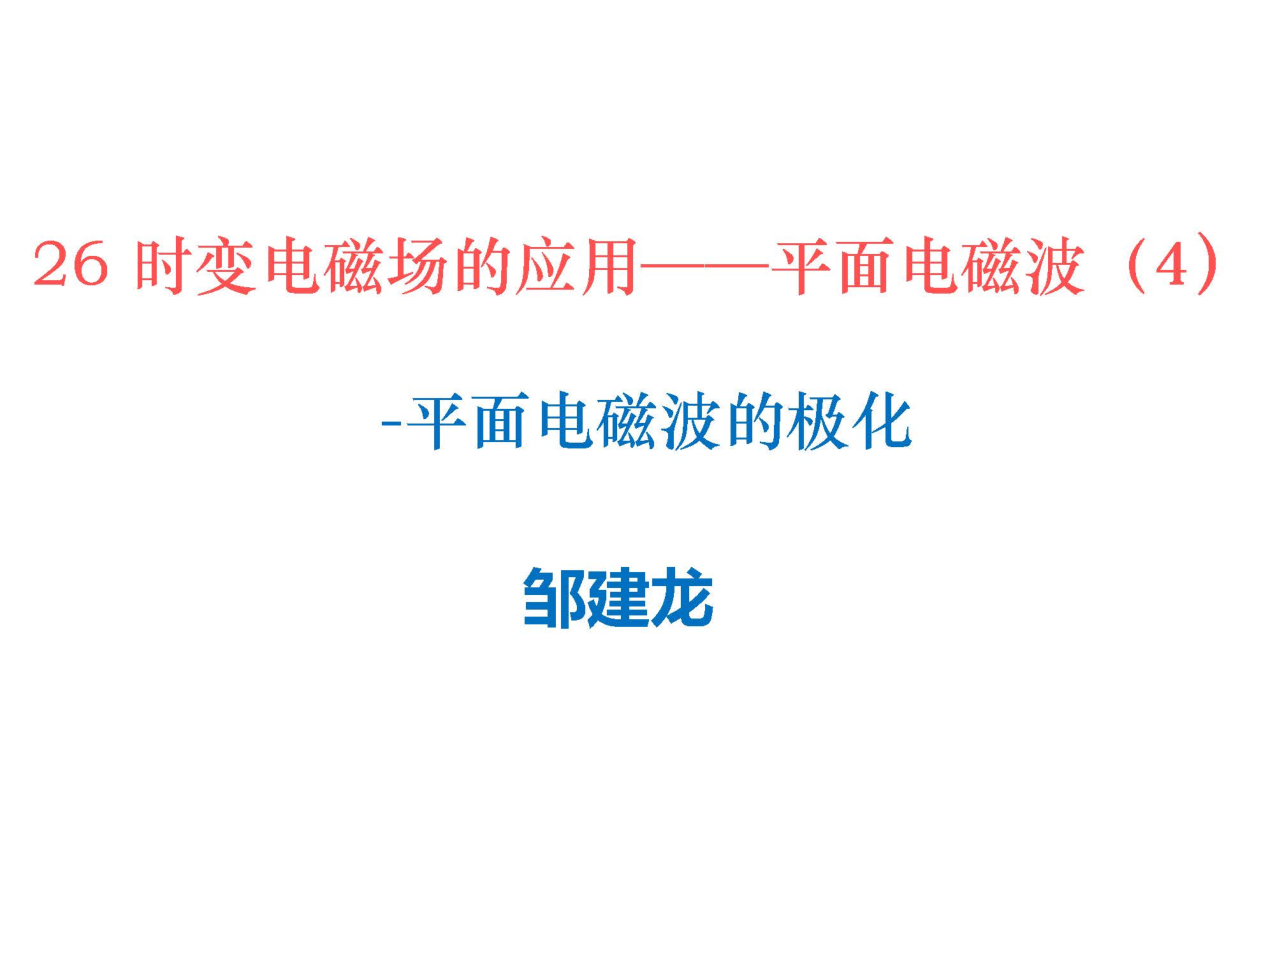
\includepdf[pages = - , nup=2x3]{content/26 时变电磁场-平面电磁波的极化(笔记).pdf}
\addcontentsline{toc}{chapter}{27 时变电磁场的应用-平面电磁波(5)-正入射、反射、透射和驻波}
\includepdf[pages = - , nup=2x3]{content/27 时变电磁场的应用-平面电磁波(5)-正入射、反射、透射和驻波(笔记).pdf}
\addcontentsline{toc}{chapter}{28 时变电磁场的应用-平面电磁波(6)-斜入射}
\includepdf[pages = - , nup=2x3]{content/28 时变电磁场的应用-平面电磁波(6)-斜入射(笔记).pdf}
\addcontentsline{toc}{chapter}{29 时变电磁场的应用-均匀传输线(1)传输线-无损耗均匀传输线方程}
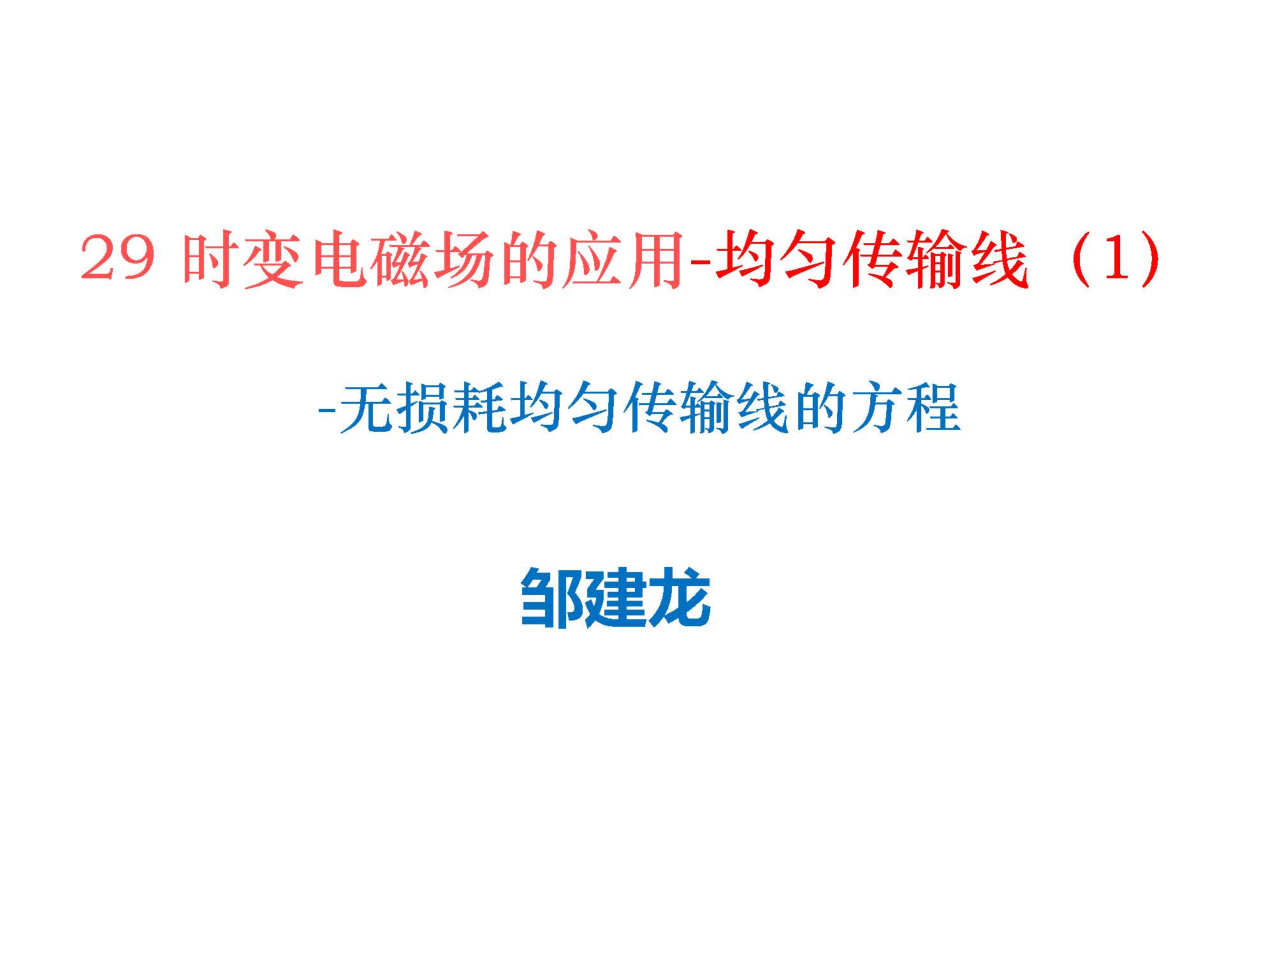
\includepdf[pages = - , nup=2x3]{content/29 时变电磁场的应用-均匀传输线(1)传输线-无损耗均匀传输线方程(笔记).pdf}
\addcontentsline{toc}{chapter}{30 时变电磁场的应用-均匀传输线(2)传输线-无损耗均匀传输线传播特性}
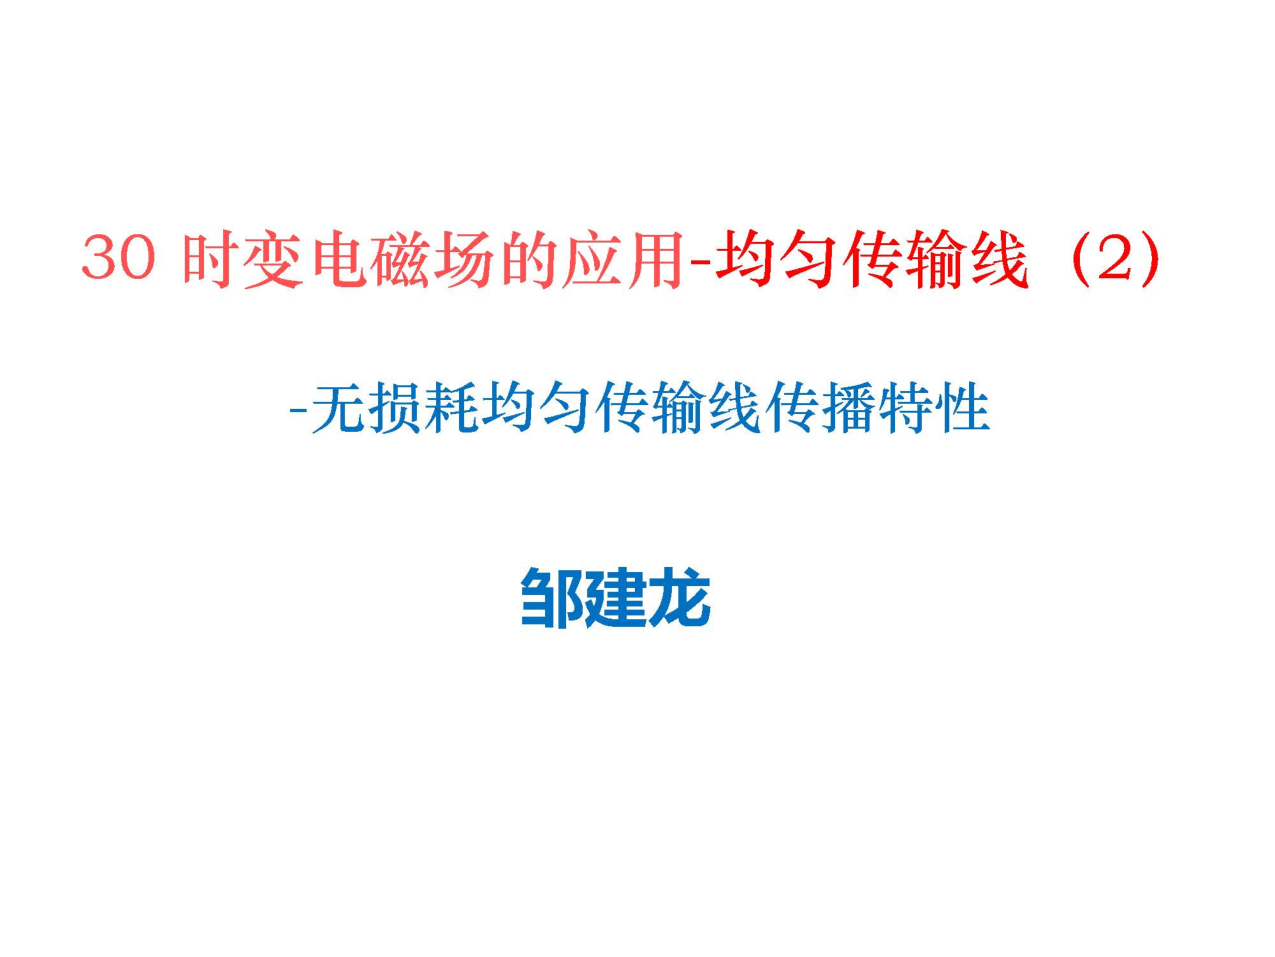
\includepdf[pages = - , nup=2x3]{content/30 时变电磁场的应用-均匀传输线(2)传输线-无损耗均匀传输线传播特性(1).pdf}
\addcontentsline{toc}{chapter}{31 时变电磁场的应用-均匀传输线(3)-无损耗均匀传输线中波的反射和透射}
\includepdf[pages = - , nup=2x3]{content/31 时变电磁场的应用-均匀传输线(3)-无损耗均匀传输线中波的反射和透射(1).pdf}
\addcontentsline{toc}{chapter}{32 时变电磁场的应用-均匀传输线(4)-无损耗均匀传输线中波的入端阻抗}
\includepdf[pages = - , nup=2x3]{content/32 时变电磁场的应用-均匀传输线(4)-无损耗均匀传输线中波的入端阻抗.pdf}
\addcontentsline{toc}{chapter}{33 时变电磁场的应用-均匀传输线(5)-无损耗均匀传输线的阻抗匹配}
\includepdf[pages = - , nup=2x3]{content/33 时变电磁场的应用-均匀传输线(5)-无损耗均匀传输线的阻抗匹配.pdf}
\addcontentsline{toc}{chapter}{34 时变电磁场的应用-均匀传输线(6)-有损耗均匀传输线}
\includepdf[pages = - , nup=2x3]{content/34 时变电磁场的应用-均匀传输线(6)-有损耗均匀传输线.pdf}
\addcontentsline{toc}{chapter}{35 时变电磁场的应用-波导(1)-波导简介与方程}
\includepdf[pages = - , nup=2x3]{content/35 时变电磁场的应用-波导(1)-波导简介与方程.pdf}
\addcontentsline{toc}{chapter}{36 时变电磁场的应用-波导(2)-矩形波导}
\includepdf[pages = - , nup=2x3]{content/36 时变电磁场的应用-波导(2)-矩形波导(笔记).pdf}
\addcontentsline{toc}{chapter}{37 时变电磁场的应用-波导(3)-介质波导}
\includepdf[pages = - , nup=2x3]{content/37 时变电磁场的应用-波导(3)-介质波导(笔记).pdf}
\addcontentsline{toc}{chapter}{38 时变电磁场的应用-谐振腔}
\includepdf[pages = - , nup=2x3]{content/38 时变电磁场的应用-谐振腔(笔记).pdf}
\addcontentsline{toc}{chapter}{39 时变电磁场的应用-天线(1)-天线简介和单元偶极子天线}
\includepdf[pages = - , nup=2x3]{content/39 时变电磁场的应用-天线(1)-天线简介和单元偶极子天线(笔记).pdf}
\addcontentsline{toc}{chapter}{40 时变电磁场的应用-天线(2)-细线天线和天线阵}
\includepdf[pages = - , nup=2x3]{content/40 时变电磁场的应用-天线(2)-细线天线和天线阵(笔记).pdf}
\addcontentsline{toc}{chapter}{41 电磁场中的能量(1)-坡印廷定理}
\includepdf[pages = - , nup=2x3]{content/41 电磁场中的能量(1)-坡印廷定理(笔记).pdf}
\addcontentsline{toc}{chapter}{42 电磁场中的能量(2)-时变电磁场的功率}
\includepdf[pages = - , nup=2x3]{content/42 电磁场中的能量(2)-时变电磁场的功率(笔记).pdf}
\addcontentsline{toc}{chapter}{43 电磁场中的能量(3)-静态场和恒定场的能量、力和功率}
\includepdf[pages = - , nup=2x3]{content/43 电磁场中的能量(3)-静态场和恒定场的能量、力和功率.pdf}
\addcontentsline{toc}{chapter}{44 准静态电磁场(1)-概念、条件和求解思路}
\includepdf[pages = - , nup=2x3]{content/44 准静态电磁场(1)-概念、条件和求解思路.pdf}
\addcontentsline{toc}{chapter}{45 准静态电磁场(2)-电准静态场与电荷驰豫}
\includepdf[pages = - , nup=2x3]{content/45 准静态电磁场(2)-电准静态场与电荷驰豫.pdf}
\addcontentsline{toc}{chapter}{46 准静态电磁场(3)-磁准静态场-集肤效应和导体交流内阻抗}
\includepdf[pages = - , nup=2x3]{content/46 准静态电磁场(3)-磁准静态场-集肤效应和导体交流内阻抗.pdf}
\addcontentsline{toc}{chapter}{47 准静态电磁场(4)-磁准静态场-邻近效应}
\includepdf[pages = - , nup=2x3]{content/47 准静态电磁场(4)-磁准静态场-邻近效应.pdf}
\addcontentsline{toc}{chapter}{48 准静态电磁场(5)-磁准静态场-涡流、涡流损耗和电磁屏蔽}
\includepdf[pages = - , nup=2x3]{content/48 准静态电磁场(5)-磁准静态场-涡流、涡流损耗和电磁屏蔽.pdf}

\includepdf[pagecommand = {\thispagestyle{empty}}, pages = - ]{lastpage.pdf}
\end{document}